\documentclass[11pt]{article}

\usepackage{aa222-jmlr2e}
\makeatother
\usepackage{lipsum}
\usepackage{pdfpages}
\usepackage{sectsty}
\usepackage{hyperref}
\usepackage{graphicx}
\usepackage{subcaption}
\usepackage{float}
\usepackage{amsmath}
\usepackage{booktabs}
\usepackage{pgfplots}
\pgfplotsset{compat=1.18}
\usepackage{natbib}
\bibliographystyle{ieeetr}

\begin{document}

\title{CME 213 Final Project Milestone 4\\
Real-Time Multi-Camera 3D Perception and Tracking for Robotics}

\author{%
\begin{center}
\begin{minipage}[t]{0.46\textwidth}\centering
\textbf{Frances Raphael}\\
{\ttfamily fraphael@stanford.edu}\\
\end{minipage}\hfill
\begin{minipage}[t]{0.46\textwidth}\centering
\textbf{Aanya Tashfeen}\\
{\ttfamily aanya@stanford.edu}\\
\end{minipage}
\end{center}
}
\maketitle

\section{Summary of Progress}

Since Milestone 3, we extended our stereo SAD implementation from a single-GPU CUDA
program to a distributed MPI+CUDA version. The new version splits the input image by
rows across MPI ranks, assigns each rank to a GPU, runs the tiled SAD kernel on each
local image slab, and gathers the final disparity map back to rank~0.

The main additions are a \texttt{main\_mpi.cu}, which handles the MPI driver logic and a script for running the scaling experiments. We kept the GPU kernels from Milestone 3
unchanged, and the MPI driver currently uses the tiled kernel because it was the
fastest version from our earlier benchmarks.

We tested the distributed version on 1, 2, and 4 ranks for two image sizes. In all
cases, the gathered disparity map matched the CPU reference on the synthetic stereo
pair. We also collected strong-scaling results on a four-GPU node. In addition, we added support for loading real stereo image pairs from
PGM files, which lets us run the same pipeline on standard stereo datasets instead
of only synthetic images.

We haven't done object tracking yet, so that is one feature of the final project that we still have to implement for the final
report.

\section{Distributed Algorithm and Data Decomposition}

We use a 1-D row decomposition across MPI ranks. For an image of height $H$ and
$P$ ranks, each rank is assigned a consecutive block of rows. Rank~$i$ owns rows
$[r_i, r_i + h_i)$, where
\[
h_i = \lfloor H/P \rfloor + [i < H \bmod P].
\]
This gives the first $H \bmod P$ ranks one extra row, so the work stays balanced
even when the image height is not exactly divisible by the number of ranks.

The main complication is that the SAD kernel does not compute each row completely
independently. Each output pixel uses a $(2R+1)\times(2R+1)$ patch, so pixels near
the top or bottom of a rank's assigned block need access to neighboring rows. To
handle this, each rank forms a local image slab that includes its owned rows plus
up to \texttt{radius} halo rows above and below. The halo bounds are clamped at the
global image boundary, so the first and last ranks do not read outside the image.

In the current implementation, we use a full-image broadcast rather than an explicit
halo exchange. Rank~0 broadcasts the full left and right images to all ranks, and
then each rank locally extracts the slab it needs. This makes the distributed logic
much simpler because every rank already has the data needed to build its halo region.
After the GPU kernel runs, only the owned rows are sent back to rank~0; the halo rows
are used for computation but are not included in the final gathered disparity map.

This approach is not communication-optimal, since every rank receives the full input
images. However, it was a reasonable first MPI implementation because the image sizes
we tested are still small enough that the broadcast overhead is manageable. For larger
images or more GPUs, the better approach would be to use \texttt{MPI\_Scatterv} to
send each rank only its assigned rows and then use \texttt{MPI\_Sendrecv} to exchange
halo rows with neighboring ranks.

We also considered a 2-D decomposition, but row decomposition fits this kernel better.
The disparity search is horizontal, so splitting the image by columns would make the
search window harder to handle near rank boundaries. With row decomposition, each
rank keeps the full image width, and the only extra data needed is a small number of
halo rows. This keeps the implementation simple while still allowing us to distribute
the main computation across multiple GPUs.

\section{MPI Implementation}

The MPI implementation is organized around two collective operations:
\texttt{MPI\_Bcast} for distributing the input images and \texttt{MPI\_Gatherv} for
collecting the final disparity map. Rank~0 either generates the synthetic stereo pair
or loads the real stereo pair from disk. It then broadcasts the image dimensions and
the full left and right image buffers to all ranks.

After the broadcast, each rank computes its row range and halo bounds. It copies the
corresponding rows into local left and right image slabs and runs the tiled CUDA SAD
kernel on those slabs. Since the local slab includes halo rows, the kernel can compute
patches correctly near the boundaries of the rank's owned region. Once the kernel
finishes, each rank copies its local disparity slab back to host memory.

The final output is assembled using \texttt{MPI\_Gatherv}. We use
\texttt{MPI\_Gatherv} instead of \texttt{MPI\_Gather} because ranks may own different
numbers of rows when $H$ is not divisible by $P$. The send count for each rank is
\texttt{local\_rows * width}, and the displacement is based on the starting row of
that rank in the full image. Each rank sends only its owned rows, starting after the
top halo region in the local disparity slab.

The current version is fully synchronous. The input broadcast completes before any GPU
work begins, and the output gather starts only after each rank has finished its CUDA
kernel and copied the result back to the host. This makes the code easier to verify
and debug, but it also means communication and data-transfer overheads are not hidden
behind computation.

MPI transfers are also staged through host memory. We do not currently use CUDA-aware
MPI, so the data path is host image buffer to device slab, then device disparity slab
back to host, then MPI gather. For the problem sizes in this milestone, this was a
reasonable tradeoff. A more optimized version would avoid some of these extra copies
by using CUDA-aware MPI or by overlapping host-device transfers with communication.


\section{CUDA Integration}

Each MPI rank selects a GPU using
\[
\texttt{cudaSetDevice(rank \% num\_devices)}.
\]
On the four-GPU node, this assigns ranks 0--3 to four separate GPUs.

The existing \texttt{GpuBuffers} wrapper from Milestone 3 is reused. The only
difference is that each rank now allocates buffers for its local slab rather than the
full image. This means memory use per GPU decreases as we add ranks.

No changes were needed inside the CUDA kernels. Each kernel already accepts an image
with arbitrary height and handles border pixels internally. For MPI, this works out
nicely because the halo rows can be passed into the kernel as part of the local slab,
and then discarded before the gather.

For timing, the CUDA kernel still uses CUDA events. In the MPI driver, we also use
\texttt{MPI\_Wtime} around the broadcast, kernel call, and gather. Since distributed
runtime is limited by the slowest rank, we report the maximum kernel time across ranks
using \texttt{MPI\_Reduce} with \texttt{MPI\_MAX}.

\section{Real Stereo Image Support}
\label{sec:realimages}

Until this milestone, our tests used a synthetic stereo pair. The left image was a
sinusoidal pattern, and the right image was generated by shifting the left image by a
known constant disparity. This was useful for correctness testing because the true
disparity was known everywhere, but it is not representative of real stereo data.

For this milestone, we added a \texttt{load\_pgm} function that reads 8-bit binary PGM images. Additionally, in the MPI version, rank~0 loads the image dimensions and pixel data, broadcasts the
dimensions first, and then broadcasts the image buffers. After that, the rest of the
pipeline is the same as for synthetic images: row decomposition, halo extraction,
CUDA kernel launch, and \texttt{MPI\_Gatherv}.

For future testing, the most useful datasets are Middlebury, KITTI, and ETH3D. These
datasets provide rectified stereo pairs, which match the horizontal-disparity
assumption used by our SAD implementation. Middlebury is useful for high-resolution
indoor scenes, KITTI is more representative of outdoor robotic perception, and ETH3D
has accurate ground truth at moderate image sizes.

\section{Correctness Testing}

We tested the distributed implementation against the CPU reference using the same
synthetic stereo setup as Milestone 3. The true disparity was fixed at
$d^* = 24$, with $D_{\max}=64$ and patch radius $R=2$.

We ran the tests on two image sizes, $480 \times 640$ and $960 \times 1280$, using
1, 2, and 4 MPI ranks. In all cases, the final gathered disparity map had
\[
\text{MAE} = 0.000 \text{ px}
\]
and a bad-pixel rate of
\[
0.00\%.
\]
This confirms that the row partitioning and halo handling are correct. In particular,
the gather does not drop or duplicate rows, and the kernel's border handling works
both at the true image boundary and at local slab boundaries.

\section{Performance, Scaling, and Profiling}

We benchmarked the MPI+CUDA version on a single node with
four GPUs and four MPI ranks, one rank per GPU. All timings are
averaged over 10 runs.

\subsection{Strong Scaling Results}

Tables~\ref{tab:scale480} and~\ref{tab:scale960} show the strong-scaling results for
the two image sizes. ``Kernel max'' is the maximum CUDA kernel time across all ranks.
``Wall'' is the total barrier-to-barrier wall clock time, including the repeated kernel launches
and host-device transfers. ``Comm'' is the measured MPI broadcast plus gather time.
Speedup and efficiency are computed using wall clock time.

\begin{table}[H]
\centering
\caption{Strong scaling for a $480\times640$ image with $D_\text{max}=64$ and $R=2$ on 4 GPUs.}
\label{tab:scale480}
\begin{tabular}{rrrrrrr}
\toprule
Ranks & Rows/rank & Kernel max (ms) & Wall (ms) & Comm (ms) & Speedup & Efficiency \\
\midrule
1 & 480 & 0.441 & 5.79 & 0.12 & 1.00 & 100\% \\
2 & 240 & 0.242 & 4.51 & 0.75 & 1.28 & 64\% \\
4 & 120 & 0.129 & 2.96 & 1.24 & 1.95 & 49\% \\
\bottomrule
\end{tabular}
\end{table}

\begin{table}[H]
\centering
\caption{Strong scaling for a $960\times1280$ image with $D_\text{max}=64$ and $R=2$ on 4 GPUs.}
\label{tab:scale960}
\begin{tabular}{rrrrrrr}
\toprule
Ranks & Rows/rank & Kernel max (ms) & Wall (ms) & Comm (ms) & Speedup & Efficiency \\
\midrule
1 & 960 & 1.749 & 21.67 & 0.43 & 1.00 & 100\% \\
2 & 480 & 0.905 & 11.96 & 1.65 & 1.81 & 90.5\% \\
4 & 240 & 0.464 & 6.90  & 2.96 & 3.14 & 78.5\% \\
\bottomrule
\end{tabular}
\end{table}

\begin{figure}[H]
\centering
\begin{subfigure}[t]{0.48\textwidth}
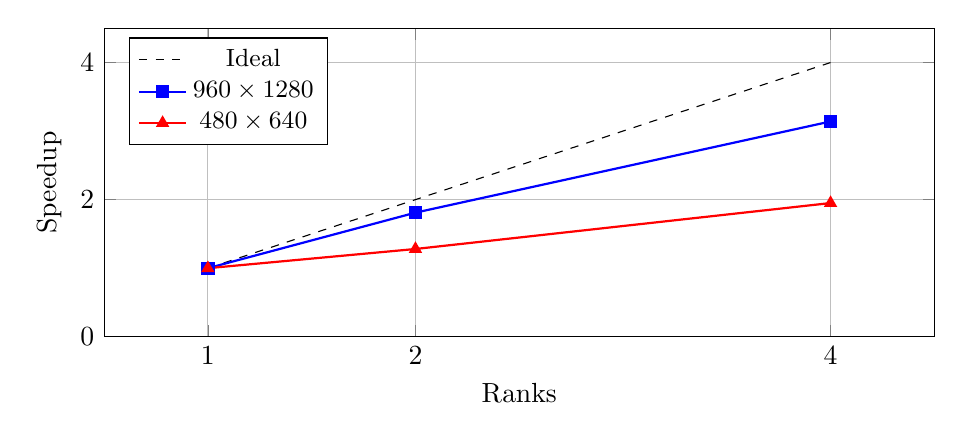
\begin{tikzpicture}
\begin{axis}[
  width=\linewidth, height=5.5cm,
  xlabel={Ranks}, ylabel={Speedup},
  xtick={1,2,4}, xmin=0.5, xmax=4.5,
  ymin=0, ymax=4.5,
  legend pos=north west, legend style={font=\small},
  grid=major,
]
\addplot[black, dashed, domain=1:4, samples=50] {x};
\addlegendentry{Ideal}
\addplot[blue, mark=square*, thick] coordinates {(1,1.00)(2,1.81)(4,3.14)};
\addlegendentry{$960\times1280$}
\addplot[red, mark=triangle*, thick] coordinates {(1,1.00)(2,1.28)(4,1.95)};
\addlegendentry{$480\times640$}
\end{axis}
\end{tikzpicture}
\caption{Speedup}
\end{subfigure}
\hfill
\begin{subfigure}[t]{0.48\textwidth}
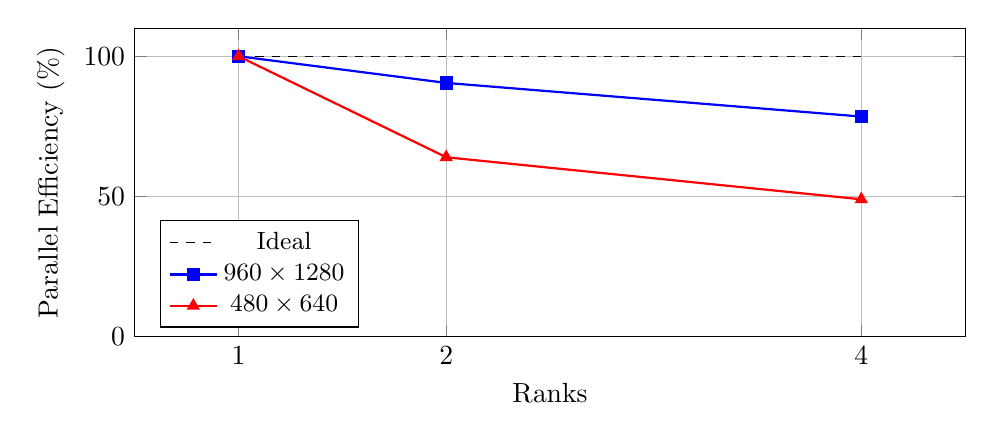
\begin{tikzpicture}
\begin{axis}[
  width=\linewidth, height=5.5cm,
  xlabel={Ranks}, ylabel={Parallel Efficiency (\%)},
  xtick={1,2,4}, xmin=0.5, xmax=4.5,
  ymin=0, ymax=110,
  legend pos=south west, legend style={font=\small},
  grid=major,
]
\addplot[black, dashed] coordinates {(1,100)(2,100)(4,100)};
\addlegendentry{Ideal}
\addplot[blue, mark=square*, thick] coordinates {(1,100)(2,90.5)(4,78.5)};
\addlegendentry{$960\times1280$}
\addplot[red, mark=triangle*, thick] coordinates {(1,100)(2,64)(4,49)};
\addlegendentry{$480\times640$}
\end{axis}
\end{tikzpicture}
\caption{Parallel efficiency}
\end{subfigure}
\caption{Strong-scaling speedup and parallel efficiency for two image sizes on 4 GPUs.}
\label{fig:scaling}
\end{figure}

\subsection{Computation vs. Communication}

Figure~\ref{fig:scaling} shows speedup and parallel efficiency curves for both image
sizes. The larger image scales much better than the smaller one. For the $960\times1280$
case, going from 1 to 4 ranks improves wall time from 21.67 ms to 6.90 ms, giving a
$3.14\times$ speedup and 78.5\% efficiency. The kernel time itself scales almost
ideally, dropping from 1.749 ms to 0.464 ms. This suggests that the CUDA work is
being split evenly across GPUs and that there is no major load imbalance.

The main reason scaling is not perfectly linear is communication. The full input
image is broadcast to every rank, and the final disparity image is gathered back to
rank~0. These communication costs do not shrink as quickly as the per-rank compute
work. As more ranks are added, each GPU gets fewer rows to process, but the full-image
broadcast and final gather are still present.

This effect is more noticeable for the $480\times640$ case. With 4 ranks, the wall
time improves from 5.79 ms to 2.96 ms, which is only a $1.95\times$ speedup. Each
rank only processes 120 rows, so the kernel is already very short. At that point,
MPI overhead and host-device transfer overhead become a much larger fraction of the
total runtime.

\subsection{Parallel Efficiency}

As seen in Figure~\ref{fig:scaling}(b), the 4-rank efficiency is 78.5\% for the larger image, but only 49\% for the smaller
image. This is the expected trend for strong scaling: when the problem size is fixed,
adding more GPUs reduces the compute work per GPU, but the fixed overheads remain.

For the large image, each rank still has enough work to keep the GPU useful, so the
parallel efficiency stays fairly high. For the small image, each local slab is too
small, and the overhead of launching kernels, transferring data, and running MPI
collectives starts to dominate. This means the smaller image is below the crossover
point where using four GPUs is clearly worth it.

\subsection{Nsight Systems Profiling}

\begin{figure}[H]
\centering
\includegraphics[width=\linewidth]{nsys_timeline.png}
\caption{Nsight Systems timeline for rank~0 on a 4-rank, $960\times1280$ run.
The two \texttt{MPI\_Bcast} calls (left) dominate the pre-kernel phase; the
actual \texttt{kernel\_tiled} execution on the GPU appears as a narrow block
in the CUDA HW row, confirming that the implementation is communication-bound.}
\label{fig:nsys}
\end{figure}

Figure~\ref{fig:nsys} shows the Nsight Systems timeline for rank~0 on a 4-rank,
$960\times1280$ run. Tables~\ref{tab:mpi_stats} and~\ref{tab:cuda_stats} summarize
the MPI and CUDA API times reported by Nsight Systems.

\begin{table}[H]
\centering
\caption{MPI operation times from Nsight Systems (rank~0, 4 ranks, $960\times1280$, 1 repeat). MPI\_Init and MPI\_Finalize are startup/teardown and not part of the algorithm.}
\label{tab:mpi_stats}
\begin{tabular}{lrrr}
\toprule
Operation & Total time & Calls & Avg \\
\midrule
MPI\_Bcast   & 4.295 ms & 3 & 1.432 ms \\
MPI\_Barrier & 2.732 ms & 4 & 0.683 ms \\
MPI\_Gatherv & 1.210 ms & 1 & 1.210 ms \\
MPI\_Reduce  & 0.069 ms & 1 & 0.069 ms \\
\bottomrule
\end{tabular}
\end{table}

\begin{table}[H]
\centering
\caption{CUDA API times from Nsight Systems (rank~0, 4 ranks, $960\times1280$, 1 repeat).}
\label{tab:cuda_stats}
\begin{tabular}{lrrr}
\toprule
Operation & Total time & Calls & Avg \\
\midrule
cudaMalloc             & 1.012 ms & 3 & 0.337 ms \\
cudaDeviceSynchronize  & 0.453 ms & 1 & 0.453 ms \\
cudaEventSynchronize   & 0.451 ms & 1 & 0.451 ms \\
cudaMemcpy             & 0.386 ms & 3 & 0.129 ms \\
cudaFree               & 0.368 ms & 3 & 0.123 ms \\
cudaLaunchKernel       & 0.176 ms & 2 & 0.088 ms \\
\bottomrule
\end{tabular}
\end{table}

The dominant algorithm-level cost is \texttt{MPI\_Bcast} at 4.295\,ms across
three calls (image dimensions, left image, right image), compared to only
1.210\,ms for \texttt{MPI\_Gatherv}. This asymmetry is expected: the broadcast
sends the full image to every rank while the gather only collects the owned rows.
On the CUDA side, host-device transfers (\texttt{cudaMemcpy}) total just 386\,µs,
and the kernel launch overhead is 176\,µs for two launches (warmup and timed).

Taken together, the profiling data confirms that GPU execution and data movement
are not the bottleneck, the MPI broadcast is, and that switching to
\texttt{MPI\_Scatterv} would have the largest impact on end-to-end runtime.

\section{Discussion of Bottlenecks}

The main bottleneck in the current distributed version is the full-image
\texttt{MPI\_Bcast}. This made the implementation much easier to debug, since every
rank has the full left and right images and can locally extract its owned rows plus
halo rows. However, it also means that each rank receives more data than it actually
needs. Each rank only needs its assigned rows and a small halo, so the natural next
step would be to replace the broadcast with \texttt{MPI\_Scatterv} and use explicit
halo exchange between neighboring ranks.

Host-device transfer is another source of overhead. Each rank copies its local slab
from the host to the GPU before launching the kernel, and then copies the disparity
slab back to the host before the gather. For this milestone, that is fine because the
goal was to get the distributed version working correctly. For a real-time pipeline,
though, these copies would become more important. A better version would use pinned
memory and \texttt{cudaMemcpyAsync}, and would try to overlap transfers with CUDA
kernel execution.

The current pipeline is also fully sequential: broadcast the inputs, copy the slab to
the GPU, run the kernel, copy the result back, and gather the output. There is no
communication-computation overlap yet. This keeps the code simple, but it also means
that MPI overhead and host-device copies show up directly in the runtime. In a more
optimized version, we would pipeline frames so that communication for one frame can
overlap with computation for another.

The scaling results show where this starts to matter. For the larger
$960\times1280$ image, the CUDA kernel scales well: the maximum kernel time drops
from 1.749\,ms at 1 rank to 0.464\,ms at 4 ranks, which is close to the ideal
$4\times$ improvement. This suggests that the row decomposition is balancing the GPU
work well. The wall-clock speedup is lower because the communication and transfer
costs do not shrink at the same rate.

For the smaller $480\times640$ image, the 4-rank speedup is much worse. Each rank
only owns 120 rows, so there is not enough work per GPU to hide the fixed overheads.
At that size, launching kernels, moving data, and running MPI collectives take a large
fraction of the total time. This suggests that the multi-GPU version is most useful
for larger images, larger disparity ranges, or more expensive stereo kernels.

Overall, the tiled SAD kernel and row decomposition were the right choices for this
milestone. The tiled kernel was already our fastest single-GPU implementation, and
the row decomposition maps cleanly onto the stereo problem because disparity search is
horizontal. A 2-D decomposition would have made the boundary logic more complicated,
especially near column boundaries, without giving an obvious benefit for this kernel.
The current implementation will likely stop scaling well once the per-rank GPU work
becomes smaller than the fixed communication and transfer costs. For our current image
sizes, that means scaling beyond 4--8 GPUs would probably not help much unless we
first reduce the broadcast volume and overlap communication with computation.

\section{Challenges and Next Steps}

The main challenge for this milestone was getting the row-slab decomposition correct.
Each rank needs halo rows to compute SAD patches near its local boundaries, but those
halo rows should not be included in the final gathered output. Most of the debugging
was around making sure the local slab indexing, gather offsets, and boundary handling
were all consistent.

The other limitation is that the current MPI version favors simplicity over
communication efficiency. Broadcasting the full image to every rank made the
implementation easier to validate, but it is also the main reason scaling will
eventually flatten.

For the final report, our next step is to replace the full-image broadcast with
\texttt{MPI\_Scatterv} plus explicit halo exchange. We also want to run larger image
sizes and larger disparity ranges, since those cases should better show the benefit of
multiple GPUs. Finally, we plan to test the PGM image-loading path on real Middlebury
or KITTI stereo pairs, and if time permits, we may still add a simple object tracking stage, but the main priority is to finish and evaluate the distributed stereo pipeline.






\end{document}